\chapter{Vertex covering}
\label{ch:cover}
\index{vertex cover}

A \emph{vertex cover} is a set of nodes touching every link, and the problem is
to find the smallest one. Section~\ref{sec:cover-intro} put it as a model ---
$x_{i}\in\{0,1\}$ on every node, the energy $\sum_{i}x_{i}$ to be minimised, and
a hard constraint $x_{i}+x_{j}\ge1$ on every link --- and it is NP-hard
\citep{karp1972}. It is also Chapter~\ref{ch:hittingset}'s hitting set at
cardinality two, which is why the two chapters are adjacent.

This chapter solves it on a chygraph. The constraint is then read over every
pair inside every complex, so a complex is a clique that has to be covered, and
what the chapter asks is what that changes: how small a cover can be when the
links arrive in triangles and cliques rather than one at a time, and how much
harder it is to find one.

Three methods answer that, in the order Chapter~\ref{ch:statmech} sets and
Chapters~\ref{ch:ising} and~\ref{ch:hittingset} follow.
Section~\ref{sec:twoconstraints} writes the interior down and reads off what a
complex transmits, which is the cavity recursion.
Section~\ref{sec:leafremoval} is leaf removal,
Sec.~\ref{sec:leafremoval-intro}'s combinatorial rule, which that recursion
turns out to describe exactly. Section~\ref{sec:coreobstruction} treats what
the rule gets stuck on --- the core --- by the LCZP map of \citet{liu2012}, a
cavity calculation carrying three states rather than one, since a node may be
settled in either of two ways or in neither.
Section~\ref{sec:fivecover} then runs the three of them over the five
structures of Fig.~\ref{fig:mappings}, one paragraph each, which is where
Chapter~\ref{ch:chygraphs}'s claim about substitution is paid out or is not.
Sections~\ref{sec:hrg}, \ref{sec:vw} and~\ref{sec:realcore} then evaluate
the map on three families of graph the chapter did not construct: hyperbolic
random graphs, whose clustering comes from the geometry; the correlated
ensemble of \citet{vazquez2003vw}, which has an arbitrary degree distribution
\emph{and} arbitrary correlation between adjacent degrees, and which is the
same hard-field map refined on a different index; and sixteen real networks.
The core appears with the triangles in all three.

Two results come out. The algorithm, the core and
Chapter~\ref{ch:hittingset}'s hard-field instability, Eq.~\eqref{eq:kc}, are
not three results sharing a number but one point computed three ways --- all
three sit at mean degree $e$, and Sec.~\ref{sec:onepoint} gives the digits. And
raising the cardinality breaks something, as it did in
Chapter~\ref{ch:hittingset}: above cardinality two the core-free branch
disappears entirely, so leaf removal never certifies anything, which is
precisely why the hard-field cover size stopped being trustworthy there.
Section~\ref{sec:corefree} proves it in three lines, and blocks the reading of
it that is too strong.

None of the ingredients is new --- leaf removal is due to \citet{bauer2001} and
the core and its transition to \citet{liu2012} --- but the identification of
all three at one point, and everything above cardinality two, is first done
here.

\section{Vertex cover as a hard-core problem}
\label{sec:twoconstraints}
\index{vertex cover}

Chapter~\ref{ch:statmech} says what to do with a model once its interior is
written down, so the chapter begins where Chapters~\ref{ch:ising}
and~\ref{ch:hittingset} began: with the interior, and with what a complex
therefore transmits.

Chapter~\ref{ch:hittingset} deferred the comparison that fixes it. Hitting set
and vertex cover minimise the same thing, $\mathcal{H}=\mu\sum_ix_i$, and differ
only in the constraint. Where Eq.~\eqref{eq:Hhs} forbids a hyperedge
with \emph{no} member taken, vertex cover of the induced graph forbids an
\emph{edge} with neither endpoint taken:
\begin{equation}
  \prod_{a}\ \prod_{\{i,j\}\subset a}
    \bigl[1-(1-x_{i})(1-x_{j})\bigr]=1.
  \label{eq:Hvc}
\end{equation}
The difference is a matter of how much of a complex may be left out. A hyperedge
is satisfied once one member is taken, so $c-1$ may be left out. Two members of
a clique are adjacent, so at most \emph{one} may.

The cavity equations differ in exactly one place, and it is again inside the
complex. Taking $i$ blocks every other member of every complex containing it ---
but a complex could only ever have contributed one member, so the cost is the
\emph{maximum} over the complex rather than the sum:
\begin{equation}
  z_{i\to a}=1-\sum_{b\ne a}\max\Bigl(0,\max_{j\in b\setminus i}z_{j\to b}\Bigr),
  \label{eq:vcz}
\end{equation}
which is one inclusion of one graph. Getting an ensemble out of it takes one
reading and two averages, and it is worth doing them slowly, because the answer
is not what Chapter~\ref{ch:hittingset} would lead one to write down.

\emph{Read the message.} $z_{i\to a}=1$ means $i$ is \emph{free} --- it may be
left out of the cover --- as seen by $a$. Everything in the sum is $0$ or $1$:
$\max_{j\in b\setminus i}z_{j\to b}$ is $1$ exactly when at least one other
member of $b$ is free, and the outer $\max(0,\cdot)$ discards the $-1$ a
complex would otherwise contribute when all of its other members are taken. So
the sum counts, and $z_{i\to a}=1$ if and only if that count is zero: $i$ is
free when no other complex \emph{blocks} it, where $b$ blocks $i$ when some
member of $b$ other than $i$ is free. That is the covering constraint read
locally --- two members of a complex are adjacent, so if $j$ is left out then
$i$ must be taken --- and writing the inner cost as a maximum rather than a sum
is what makes blocking one yes-or-no event per complex instead of a count of
them. A yes-or-no event per complex is what a generating function can average.

\emph{Average inside one complex.} Let $\sigma_{l}$ be the probability that a
node reached along an inclusion into a layer-$l$ complex is free. Enter a
layer-$l$ complex at $i$ and look at its other $c_{l}-1$ members. By the reading
above, the complex fails to block $i$ exactly when \emph{none} of them is free.
On a treelike chygraph the branches behind those members meet only at the
complex, so the $c_{l}-1$ events are independent and their probabilities
multiply. Write $\tau_{l}$ for the result:
\[
  \tau_{l}=\underbrace{(1-\sigma_{l})\cdots(1-\sigma_{l})}_{c_{l}-1}
          =(1-\sigma_{l})^{\,c_{l}-1}.
\]

\emph{Average over the complexes at a node.} Now $i$ itself. It is free when
every one of its other complexes fails to block it, each independently with
probability $\tau$, and how many others it has is the excess chy-degree of
Sec.~\ref{sec:ensembles} --- excess, because the inclusion $i$ was reached
along does not count again. Averaging $\tau^{n}$ over that count is what
$\bar\Phi$ does by definition, $\bar\Phi^{(m)}(\tau)=\sum_{n}\bar p^{(m)}_{n}
\tau^{n}$, so $\sigma_{m}=\bar\Phi^{(m)}(\tau)$. Collecting the two averages,
\begin{equation}
  \sigma_{m}=\bar\Phi^{(m)}(\tau),
  \qquad
  \tau_{l}=(1-\sigma_{l})^{\,c_{l}-1}.
  \label{eq:vc}
\end{equation}
Section~\ref{sec:treelike}'s condition is used twice
over, in two different places: once inside a complex, to multiply the
$c_{l}-1$ members, and once across the complexes at a node, to evaluate
$\bar\Phi$. It is the first of the three assumptions Sec.~\ref{sec:assumes}
lists, and it is carrying both steps here.

\emph{Where the complement went.} Chapter~\ref{ch:hittingset} writes
$\tau_{l}=\sigma_{l}^{\,c_{l}-1}$ and then $\sigma_{m}=\bar\Phi^{(m)}(1-\tau)$,
with the complement outside; here it is inside, and $\tau$ means the opposite
thing. The reason is one word. A hyperedge forces the node it is entered from
when \emph{all} of its other members are free, since then nobody else will
satisfy it. A clique forces when \emph{any} other member is free, since that one
member is already an uncovered edge. All against any is where the complement
moves, and it is Eq.~\eqref{eq:Hvc} against Eq.~\eqref{eq:Hhs} arriving in the
recursion.

At $c=2$ Eq.~\eqref{eq:vc} collapses onto Eq.~\eqref{eq:hs}, as it must --- both
return the Weigt--Hartmann cover size, to nine digits, along code paths that
share nothing. Both are reached from one handle: \code{Chygraph.\allowbreak clique\_\allowbreak cover}
returns the object whose \code{tau} is the interior factor $\tau$ and whose
\code{solve} is the map, and it reaches its fixed point by the bracket of
Sec.~\ref{sec:hard} rather than by plain iteration, both maps being
order-reversing. The algebra is in \code{cover.\allowbreak CliqueCover}.

And both are hard-field maps, so Sec.~\ref{sec:hardfail} applies to
Eq.~\eqref{eq:vcz} unchanged. On isolated triangles, where every vertex sits at
$z=0$, it returns $1/2$ against a true $2/3$. That is the mirror image of
Chapter~\ref{ch:hittingset}'s counterexample: the same defect, a different
problem, a different true answer --- and the same wrong one, because $1/2$ is
what the half rule always returns when everything is degenerate.

\section{Leaf removal, and what it certifies}
\label{sec:leafremoval}
\index{leaf removal}

Equation~\eqref{eq:vc} is the map. It has a combinatorial counterpart, and the
rest of the chapter is about what the two have to do with each other: on sparse
random graphs there is an algorithm that solves minimum vertex cover exactly,
most of the time, in linear time, NP-hardness notwithstanding.

\emph{Leaf removal.} Find a vertex of degree one --- a leaf. Its single
neighbour can be put in the cover with no loss: some minimum cover contains that
neighbour, because covering the leaf's edge costs one vertex either way and the
neighbour may cover others besides. So take the neighbour, delete both, and
repeat.

Two things about this. It is exact --- every step is forced, not heuristic --- so
if the graph is consumed entirely, the cover produced is provably minimum. And
it is a purely local rule, which is why a cavity treatment can follow it.

What it cannot do is proceed once no leaf is left. The residue at that point is
the \emph{core}, and on the core the algorithm has nothing to say: covering it
is back to being hard. Core percolation is therefore the obstruction to solving
vertex cover rather than a separate problem standing beside it, and that is why
it belongs in the same chapter. Figure~\ref{fig:leafremoval} is the rule
and what stops it.

\begin{figure}[t]
\centering
\begin{adjustbox}{max width=\linewidth}
\begin{tikzpicture}[x=1cm,y=1cm]
% Leaf removal, three frames. A leaf's NEIGHBOUR is taken; both are deleted.
\foreach \f/\lab in {0/{a leaf, and\\ its neighbour},
                     1/{take the neighbour,\\ delete both},
                     2/{no leaf left:\\ the residue is the core}}{
  \node[lb,anchor=north,align=center,text width=3.0cm]
    at (\f*3.9+0.9,-1.25) {\lab};
}
% --- frame 1
\begin{scope}
  \node[nd] (p0) at (0,0.75) {};
  \node[hub] (q0) at (0.9,0.35) {};
  \node[nd] (r0) at (1.8,0.75) {};
  \node[nd] (s0) at (1.35,-0.45) {};
  \node[nd] (t0) at (0.45,-0.45) {};
  \draw[lnk] (p0)--(q0) (q0)--(r0) (r0)--(s0) (s0)--(t0) (t0)--(r0);
  \node[lb,anchor=east] at (-0.12,0.75) {leaf};
\end{scope}
% --- frame 2
\begin{scope}[xshift=3.9cm]
  \node[nd,draw=black!25] (p1) at (0,0.75) {};
  \node[nd,draw=black!25] (q1) at (0.9,0.35) {};
  \node[nd] (r1) at (1.8,0.75) {};
  \node[nd] (s1) at (1.35,-0.45) {};
  \node[nd] (t1) at (0.45,-0.45) {};
  \draw[lnk,draw=black!18] (p1)--(q1) (q1)--(r1);
  \draw[lnk] (r1)--(s1) (s1)--(t1) (t1)--(r1);
\end{scope}
% --- frame 3
\begin{scope}[xshift=7.8cm]
  \node[hub] (r2) at (1.8,0.75) {};
  \node[hub] (s2) at (1.35,-0.45) {};
  \node[hub] (t2) at (0.45,-0.45) {};
  \draw[lnk] (r2)--(s2) (s2)--(t2) (t2)--(r2);
  \begin{scope}[on background layer]
    \node[cx,fit=(r2)(s2)(t2)] {};
  \end{scope}
\end{scope}
\end{tikzpicture}
\end{adjustbox}
\caption{\textbf{Vertex covering leaf removal.} A vertex of degree one is a
leaf; some minimum cover contains its \emph{neighbour}, so the neighbour is
taken (dark) and both are deleted. Repeating consumes the graph, and if it
consumes all of it the cover produced is provably minimum. Here it does not: the
triangle has no leaf, and the residue is the core --- the structure on which the
algorithm has nothing to say, and which the rest of the chapter is about.}
\label{fig:leafremoval}
\end{figure}

\section{The core as an obstruction}
\label{sec:coreobstruction}
\index{core}
\index{core percolation|textbf}

Run leaf removal on the cavity branch and ask what a node reached along an
inclusion ends up as. There are three answers, not two: leaf-ready ($L$),
deleted ($D$), or core-side ($C$). Percolation had two answers and got a scalar;
this has three, and needs a message with three components.

The branch is Sec.~\ref{sec:cavity}'s construction. Take the inclusion of a node
$i$ into a complex $a$, remove $a$, and what still hangs off $i$ --- its other
complexes, and everything reachable through them --- is the cavity branch.
Running the algorithm there and nowhere else makes the outcome a property of the
branch alone, which is what lets it travel along the inclusion as a message.

The three states are the three things the branch can tell $a$
(Fig.~\ref{fig:cavitybranch}).
\emph{Leaf-ready}: the branch consumed itself and left $i$ holding nothing else,
so $i$ is a leaf as far as $a$ is concerned and $a$ may take it.
\emph{Deleted}: some other complex has already taken $i$, which is therefore
not there to be counted. \emph{Core-side}: the algorithm stalled on the branch
with $i$ still holding two or more live inclusions, and $a$ cannot resolve it.
The first two are both settled and they act on $a$ in opposite directions --- one
offers it a leaf, the other removes a member --- which is why they cannot be
collapsed into a single number the way percolation's two answers could.

The three-state cavity treatment of core percolation on graphs is due to
\citet{liu2012}, and is called the \emph{LCZP map} here, after Liu, Cs\'oka,
Zhou and P\'osfai. What follows carries it to complexes, so
Eq.~\eqref{eq:core} is the LCZP map on a chygraph. The letters here are
this book's: $\psi$ and $\delta$ are written $\alpha$ and $\beta$ in that paper
--- their $\alpha$-removable and $\beta$-removable --- and both letters are
spoken for elsewhere in this book, $\alpha$ being
Chapter~\ref{ch:satisfiability}'s clause density and $\beta$ the inverse
temperature throughout Part~III.

Writing $(\psi,\delta,\gamma)$ for the probabilities of the three states
--- leaf-ready, deleted, core --- the chy-degree step is
\begin{equation}
  \psi_{m}=\bar\Phi^{(m)}(\zeta),
  \qquad
  \delta_{m}=1-\bar\Phi^{(m)}(1-\xi),
  \label{eq:core}
\end{equation}
and the intra-complex step is solved exactly, as Sec.~\ref{sec:downstep} always
does. Two equations carry three states because the third is fixed by
normalisation, $\gamma_{m}=1-\psi_{m}-\delta_{m}$: a node is leaf-ready,
deleted, or --- failing both --- core-side. A branch with no core is therefore
$\psi+\delta=1$, which is the form Sec.~\ref{sec:corefree} puts to the map.

The two quantities it supplies, $\zeta$ and $\xi$, are what a complex does to a
node entering it. Enter a layer-$l$ complex through one member and look at the
other $c_{l}-1$. With $n$ of them still live, every live member has
clique-degree exactly $n$ inside the complex, so two events matter and no
others.

\emph{The complex leaves the entering node free to be a leaf} only when it
offers nothing at all --- when every one of the other $c_{l}-1$ members is
already deleted --- so $\zeta_{l}=\delta_{l}^{\,c_{l}-1}$.

\emph{The complex forces the entering node out} only when exactly one other
member is live and leaf-ready. With two or more live members the entering node
is not a leaf of that complex and the complex decides nothing. There are
$c_{l}-1$ ways to choose which member is the live one, so
$\xi_{l}=(c_{l}-1)\,\delta_{l}^{\,c_{l}-2}\psi_{l}$.

At $c_{l}=2$ these degenerate to $\zeta_{l}=\delta_{l}$ and $\xi_{l}=\psi_{l}$,
returning the graph recursion $\psi=\bar\Phi(\delta)$, $\delta=1-\bar\Phi(1-\psi)$. The whole of it
--- the three states, the two intra-complex quantities and the fixed point --- is
\code{Chygraph.\allowbreak core}, whose \code{solve} iterates monotonically from
zero because, unlike Eq.~\eqref{eq:vc}, this map is order-preserving; the
algebra is in \code{core.\allowbreak CorePercolation}.




\begin{figure}[t]
\centering
\begin{adjustbox}{max width=\linewidth}
\begin{tikzpicture}[
  gone/.style={draw=black!22,fill=white,text=black!30},
  gonel/.style={draw=black!22},
]
% ============================= (a) leaf-ready
\begin{scope}
  \node[tb,anchor=west] at (-0.55,3.15) {(a) leaf-ready};
  \node[cpx,draw=black!55,dashed] (aA) at (1.05,2.55) {};
  \node[lb,anchor=west] at (1.28,2.55) {$a$};
  \node[atm] (iA) at (1.05,1.65) {};
  \node[lb,anchor=east] at (0.86,1.65) {$i$};
  \draw[incd] (aA)--(iA);
  \node[cpx,gone] (b1A) at (0.30,0.80) {};
  \node[cpx,gone] (b2A) at (1.80,0.80) {};
  \node[atm,gone,fill=white] (j1A) at (0.30,0.05) {};
  \node[atm,gone,fill=white] (j2A) at (1.80,0.05) {};
  \draw[gonel] (iA)--(b1A) (iA)--(b2A) (b1A)--(j1A) (b2A)--(j2A);
  \node[lb,anchor=west,align=left] at (-0.55,-0.85)
    {the branch consumed itself:\\ $i$ holds nothing else, so $a$\\ may take it as a leaf};
\end{scope}
% ============================= (b) deleted
\begin{scope}[xshift=4.35cm]
  \node[tb,anchor=west] at (-0.55,3.15) {(b) deleted};
  \node[cpx,draw=black!55,dashed] (aB) at (1.05,2.55) {};
  \node[lb,anchor=west] at (1.28,2.55) {$a$};
  \node[atm,gone,fill=white] (iB) at (1.05,1.65) {};
  \node[lb,anchor=east] at (0.86,1.65) {$i$};
  \draw[incd,gonel] (aB)--(iB);
  \node[cpx] (b1B) at (0.30,0.80) {};
  \node[lb,anchor=east] at (0.11,0.80) {$b$};
  \node[cpx,gone] (b2B) at (1.80,0.80) {};
  \node[atm] (j1B) at (0.30,0.05) {};
  \node[lb,anchor=east] at (0.11,0.05) {$j$};
  \node[atm,gone,fill=white] (j2B) at (1.80,0.05) {};
  \draw[inc] (b1B)--(j1B);
  \draw[gonel] (iB)--(b2B) (b2B)--(j2B);
  \draw[msg] (b1B) -- (iB);
  \node[lb,anchor=west,align=left] at (-0.55,-0.85)
    {$b$ holds one live leaf-ready\\ member, so it takes $i$:\\ $i$ is gone before $a$ sees it};
\end{scope}
% ============================= (c) core-side
\begin{scope}[xshift=8.7cm]
  \node[tb,anchor=west] at (-0.55,3.15) {(c) core-side};
  \node[cpx,draw=black!55,dashed] (aC) at (1.05,2.55) {};
  \node[lb,anchor=west] at (1.28,2.55) {$a$};
  \node[atm] (iC) at (1.05,1.65) {};
  \node[lb,anchor=east] at (0.86,1.65) {$i$};
  \draw[incd] (aC)--(iC);
  \node[circle,draw=black!70,line width=.5pt,minimum size=4.6mm,inner sep=0pt]
        at (1.05,1.65) {};
  \node[cpx] (b1C) at (0.30,0.80) {};
  \node[cpx] (b2C) at (1.80,0.80) {};
  \node[atm] (j1C) at (0.30,0.05) {};
  \node[atm] (j2C) at (1.80,0.05) {};
  \draw[inc] (iC)--(b1C) (iC)--(b2C) (b1C)--(j1C) (b2C)--(j2C);
  \node[lb,anchor=west,align=left] at (-0.55,-0.85)
    {two live inclusions survive:\\ the algorithm stalls and\\ $a$ cannot resolve $i$};
\end{scope}
\end{tikzpicture}
\end{adjustbox}
\caption{\textbf{The cavity branch and the LCZP map.} Drawn
as inclusions in the vocabulary of Sec.~\ref{sec:drawing}: filled circles are
atoms, rectangles complexes, a line is membership. In each panel the complex
$a$ is the one arrived through and is removed --- drawn dashed --- and what
hangs below $i$ is the cavity branch. Leaf removal is run on that branch and
nowhere else, which is what makes the outcome a property of the branch and so a
message on the inclusion $i\to a$. Pale grey is what the algorithm has already
stripped. The three outcomes are not two: (a) and (b) are both settled and act
on $a$ in opposite directions, one offering it a leaf and the other removing a
member, which is why the LCZP map carries three numbers where
Chapter~\ref{ch:percolation} carried one.}
\label{fig:cavitybranch}
\end{figure}

Unlike Eq.~\eqref{eq:hs} this map is order-\emph{preserving}, so monotone
iteration from zero suffices and none of Sec.~\ref{sec:hard}'s bracketing
apparatus is needed. That is the distinction Sec.~\ref{sec:fixedpoint} drew, put
to use: the two maps live on the same chygraph and differ in the signs of their
entries, and the sign decides which solver applies.

\paragraph{The branch is a device and not a step of the algorithm.} Leaf removal
does not remove a complex and restart; it peels the whole object at once, and
Sec.~\ref{sec:leafremoval}'s rule never mentions a cavity. What the branch does
is turn that global peeling into a local recursion, and it is exactly where the
treelike assumption enters: cutting $a$ is taken to leave the rest of $i$'s
neighbourhood self-contained. Where it does not --- where the branch closes on
itself by some other route --- the LCZP map is predicting the output of an
algorithm that will not do what the recursion says, and the algorithm is the one
that is right, since Sec.~\ref{sec:leafremoval}'s exchange argument holds on any
graph. Sections~\ref{sec:hrg} and~\ref{sec:realcore} measure the size of that
gap; it is the whole of the difference between their measured and chygraph
columns.

\section{On a graph: one point, three names}
\label{sec:onepoint}

At $c=2$ the LCZP map has threshold $\bar\Phi'(1-\psi)=1$, which for
Poisson chy-degree is
\begin{equation}
  \ave{k}=e.
\end{equation}
Below it the core is empty and leaf removal certifies a minimum cover; above it
the core is extensive and the algorithm stalls. This is the Bauer--Golinelli
threshold \citep{bauer2001}.

It is also Eq.~\eqref{eq:kc} at $c=2$: the loss of stability of
Chapter~\ref{ch:hittingset}'s hard-field map. And it is the accepted
replica-symmetry-breaking point for vertex cover on Poisson graphs
\citep{weigt2000}. Computed independently, the first two agree to
$2.5\times10^{-10}$, which is a consistency check rather than a coincidence:
they are the same point reached by two routes.


In words, and this is why the three subjects share a chapter. \emph{Leaf removal certifies a
cover exactly when there is no core; there is no core exactly when the
hard-field map is stable; and the hard-field map is stable exactly where the
integer messages carry the whole answer.} Three statements, one condition.

\paragraph{Over several layers.} The threshold above is the one-layer form,
and the general one is worth writing down because three of
Fig.~\ref{fig:mappings}'s five structures carry more than one layer. The
core-free branch is a \emph{vector}, $\psi_{m}=\bar\Phi^{(m)}(1-\psi)$ with one
entry per layer, since a node reached along a layer-$m$ inclusion is
size-biased in layer $m$ alone and two layers share a $\psi$ only when they are
statistically alike. Linearising Eq.~\eqref{eq:core} there gives a Jacobian
$\bigl(\begin{smallmatrix}0&A\\A&0\end{smallmatrix}\bigr)$ --- at $c=2$ the
$\psi$ row moves only with $\zeta=\delta$ and the $\delta$ row only with
$\xi=\psi$ --- so its spectrum is $\pm$ that of
\begin{equation}
  A_{ml}=\frac{\partial\bar\Phi^{(m)}}{\partial x_{l}}\bigg|_{x=1-\psi},
  \qquad\text{and the core appears at}\quad \rho(A)=1.
  \label{eq:corethresh}
\end{equation}
Those eigenvalues are real: $A_{ml}$ is $\partial^{2}\Phi/\partial
x_{m}\partial x_{l}$, symmetric, divided by the mean layer-$m$ chy-degree. At
$L=1$ it is $\bar\Phi'(1-\psi)=1$ again. This is
\code{core\_\allowbreak free\_\allowbreak spectral}.

For Poisson layers it collapses much further. Every $\bar\Phi^{(m)}$ is then
$\Phi$ itself, so $\psi$ is common to the layers and $A_{ml}=\kappa_{l}\psi$
does not depend on $m$: $A$ has rank one, $\rho(A)=\psi\sum_{l}\kappa_{l}$, and
with $\psi=e^{-\psi\sum_{l}\kappa_{l}}$ the threshold is
\begin{equation}
  \sum_{l}\kappa_{l}=e.
  \label{eq:sumkappae}
\end{equation}
The \emph{total} chy-degree, however it is split. So the multiplex and the
interacting graphs of Fig.~\ref{fig:mappings} sit at the graph's own threshold
rather than somewhere else, and adding a link type moves nothing;
Eq.~\eqref{eq:sumkappae} is checked against Eq.~\eqref{eq:corethresh} to
$2\times10^{-10}$ at one, two, three and five layers. Layers move the point only
when they differ in \emph{shape} and not merely in mean. A multiplex of a
diluted matching layer and a Poisson layer cores at total $\ave{k}=2.6196$,
against $2.6994$ for the single graph with the same pooled degree distribution
--- the difference being the degree correlation multiplexing imposes on the
matching layer's own links, which pooling destroys.

\paragraph{Which replica-symmetry-breaking point.} The first of
Sec.~\ref{sec:onestep}'s two, and it is worth being explicit because the
distinction costs a chapter elsewhere. This is where the solution space
\emph{shatters} --- where clusters appear and the core along with them --- and
not where minimum covers run out; covers exist on both sides of $e$, and what
changes is whether they form one cluster or many. Locating it here needs no
survey: the core is a percolation problem and the LCZP map solves it by
algebra. Section~\ref{sec:colouring-sp} reaches the same class of point for
colouring by the other route, as the density at which its surveys stop being
trivial, and pays a population dynamics for it.

What lies past $e$ this chapter does not compute. That is the complexity of
Eq.~\eqref{eq:sigmagen}, and Chapters~\ref{ch:colouring}
and~\ref{ch:satisfiability} are where the book carries it out --- for colouring
and satisfiability, not for this family, whose own one-step answer
Sec.~\ref{sec:hsrsb} states the cost of and leaves open.

\section{Above cardinality two the core-free branch disappears}
\label{sec:corefree}
\index{core}

Raising the cardinality changes the picture abruptly.

A core-free branch means $\gamma=0$, that is $\psi+\delta=1$. Substituting
Eq.~\eqref{eq:core},
\[
  \bar\Phi^{(m)}(\zeta)+1-\bar\Phi^{(m)}(1-\xi)=1,
\]
and since $\bar\Phi$ is a power series with non-negative coefficients, hence
strictly increasing, this requires $\zeta=1-\xi$ in every layer. With
$\psi=1-\delta$ that is
\[
  f(\delta)\equiv(c-1)\delta^{\,c-2}-(c-2)\delta^{\,c-1}-1=0.
\]
The polynomial factors, and the factorisation is the whole argument:
\begin{equation}
  f(\delta)=-(1-\delta)^{2}\sum_{j=0}^{c-3}(j+1)\,\delta^{\,j}.
  \label{eq:factored}
\end{equation}
At $c=2$ the sum is empty and $f\equiv0$: the condition is an \emph{identity},
and the core-free branch exists at every chy-degree below threshold. At $c\ge3$
every coefficient of the sum is strictly positive, so $f(\delta)<0$ on $[0,1)$
and $f(1)=0$. The only root is $\delta=1$, forcing $\psi=0$. The predicate is \code{has\_\allowbreak core\_\allowbreak free\_\allowbreak branch} on
that same object, and it returns true exactly when every cardinality is two.

So a chygraph carrying any layer of cardinality three or more has no core-free
branch at all, at any density. Leaf removal never certifies a cover there.

Figure~\ref{fig:core} draws it. At $c=2$ there is a transition at $e$; at $c=3$
and above there is no transition, and the two curves lie exactly on top of each
other because for a pure clique network of cardinality three or more the core is
$1-e^{-\ave{k}}$ --- every vertex that is in any complex at all. Cardinality
past three changes nothing: the obstruction is not a matter of degree.

\begin{figure}[t]
\centering
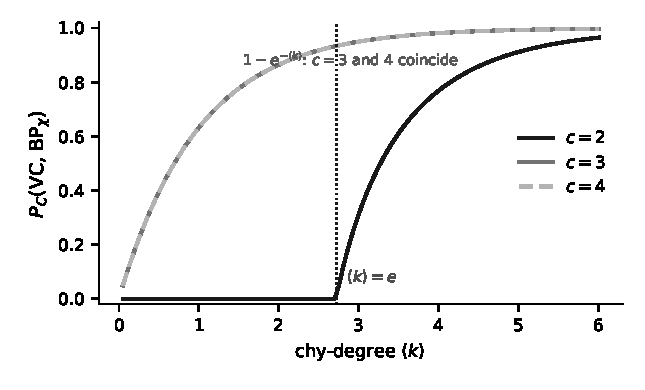
\includegraphics[width=0.88\linewidth]{figs/fig-core.pdf}
\caption{\textbf{The core-free branch and its disappearance.} Core fraction
$P_{C}(\mathrm{VC},\chi)$ --- take a chy-degree-one atom together
with the complex holding it, and what survives is the core --- against
chy-degree, for pure clique networks. At cardinality two there is a
transition at $\ave{k}=e$, below which the core is empty and leaf removal
certifies a minimum cover. At cardinality three and above there is no
transition: Eq.~\eqref{eq:factored} forbids the core-free branch, and the core
is $1-e^{-\ave{k}}$, every non-isolated vertex. The $c=3$ and $c=4$ curves
coincide exactly. Generated by \code{figs/\allowbreak cover.\allowbreak py}.}
\label{fig:core}
\end{figure}

This closes a loop. Section~\ref{sec:hardfail} said the hard-field cover size is
exact at cardinality two and an approximation above it, and appealed to
certification without proving it. Equation~\eqref{eq:factored} is the proof, and
it is a property of the LCZP map rather than an assumption imported from
elsewhere: the cover size of Eq.~\eqref{eq:hs} can be believed exactly when
the LCZP map admits $\gamma=0$, and both hold only at $c=2$.

\paragraph{A reading to block.} The result does \emph{not} say that a complex
survives leaf removal whole. Leaf removal deletes a leaf's \emph{neighbour}, and
a triangle carrying one pendant edge per vertex has an empty core. What the
algebra gives is only that the core cannot vanish identically --- not that it is
large. Add a triangle layer of chy-degree $10^{-3}$ to a Poisson link layer of
chy-degree $1$ and the predicted core is $1.8\times10^{-4}$: non-zero, as
Eq.~\eqref{eq:factored} requires, and of no practical consequence whatever. The
statement is about a branch of a fixed point, and a statement about a branch is
not a statement about a magnitude.

\paragraph{How small, exactly.} The magnitude has a closed form, and it is
worth having because Sec.~\ref{sec:realcore} meets it four times in data. Put a
clique layer of cardinality $c$ and chy-degree $\kappa_{c}$ on a link layer and
expand Eq.~\eqref{eq:core} to first order in $\kappa_{c}$. Writing $\psi_{0}$
for the link layer's own leaf-ready probability, $\psi_{0}=\bar\Phi(1-\psi_{0})$,
and $\delta_{0}=1-\psi_{0}$,
\begin{equation}
  P_{C}(\mathrm{VC},\chi)\simeq\kappa_{c}\,\psi_{0}
    \Bigl[1-\delta_{0}^{\,c-1}-(c-1)\,\psi_{0}\,\delta_{0}^{\,c-2}\Bigr].
  \label{eq:smallcore}
\end{equation}
The bracket is $1-\zeta-\xi$ evaluated on the link background: the chance that
the clique neither leaves the entering node free nor deletes it, which is the
chance it leaves it core-side. At $c=2$ it is zero identically, as it must be,
and at $c=3$ the whole expression is $\kappa_{\triangle}\psi_{0}^{3}$ --- one
triangle in the core exactly when all three of its branches are leaf-ready,
which is the combinatorial statement one would write down directly. At link
chy-degree $1$ and $\kappa_{\triangle}=10^{-3}$ it gives $1.824\times10^{-4}$,
the number quoted above.

Two things follow, and they are the point of writing it out. The core is
\emph{linear} in the clique density with a bounded slope, so
Eq.~\eqref{eq:factored} constrains a slope and not a magnitude --- which is the
previous paragraph, now with a coefficient. And Eq.~\eqref{eq:smallcore} does
not diverge at $\ave{k}=e$. The cavity $\gamma$ does, carrying a factor
$1/[1-\bar\Phi'(1-\psi_{0})]$, but the core fraction multiplies it by the same
factor and the two cancel exactly. So the transition a link layer has at $e$
does not turn into a divergence when a few triangles are added to it. It turns
into nothing at all, and Eq.~\eqref{eq:smallcore} passes through $e$ without
registering it.

\paragraph{Where the three names separate.} Section~\ref{sec:onepoint}'s
identification is a statement about $c=2$, and above $c=2$ its three names come
apart. The core has no threshold at all, which is what
Eq.~\eqref{eq:factored} has just said. The two hard-field maps still have one
each, and those two are no longer the same point either. Eliminating
$\kappa$ between the Poisson fixed point of Eq.~\eqref{eq:vc},
$\sigma=e^{\kappa(u^{c-1}-1)}$ with $u=1-\sigma$, and its instability
$\kappa(c-1)\sigma u^{c-2}=1$ leaves one transcendental equation in $\sigma$
alone:
\begin{equation}
  \ln\sigma=\frac{u^{\,c-1}-1}{(c-1)\,\sigma\,u^{\,c-2}},
  \qquad
  \ave{k}_{c}=\frac{1}{\sigma\,u^{\,c-2}},
  \label{eq:vcinstab}
\end{equation}
where $\ave{k}_{c}=\kappa(c-1)$ is the induced mean degree. It returns $e$ at
$c=2$, and then $4.7836$, $7.0871$, $9.5736$ at $c=3,4,5$: covering a clique
network gets harder, in neighbours per node, as the cliques grow. Read the same
way Chapter~\ref{ch:hittingset} reads Eq.~\eqref{eq:kc}, the hitting-set point
does not move at all --- $\ave{k}(c-1)=e$ for every cardinality. So the two
instabilities coincide at $c=2$ and separate immediately above it, and three
names for one point is precisely what cardinality two buys.

\section{Structured networks}
\label{sec:fivecover}

Chapter~\ref{ch:chygraphs} claimed that a calculation done once on a chygraph
is a calculation done for all five structures of Fig.~\ref{fig:mappings}, and
that specialising it is substitution rather than rederivation. The chapter is
now far enough along to pay that out. Section~\ref{sec:hsfive} does the same
for hitting set, and the two lists do not split alike: that section says where
they differ and why. What follows is the five, in
Sec.~\ref{sec:everything}'s order and under its names. None of it is a new
calculation: every entry is Eq.~\eqref{eq:vc} or Eq.~\eqref{eq:core} with a
list of cardinalities substituted, and Table~\ref{tab:five} is what comes back.

One number decides the whole table. Equation~\eqref{eq:factored} says the
core-free branch survives exactly when every layer has cardinality two, so the
five split two against three, and which side a structure falls on is a property
of its layer list and of nothing else --- not of its density, not of its degree
distribution, not of how many layers it carries.

\begin{table}[t]
\centering\small
\begin{adjustbox}{max width=\linewidth}
\begin{tabular}{lccrrc}
\hline\hline
structure & $c$ & threshold & $P_{C}$ & cover & certified\\
\hline
A graph & $2$ & $\ave{k}=e$ & 0.0000 & 0.3920 & yes\\
A hypergraph & $3$ & none & 0.6321 & 0.3426$^{*}$ & no\\
A multiplex network & $2,2$ & $\ave{k}=e$ & 0.0000 & 0.3920 & yes\\
Interacting graphs & $2,2,2$ & $\ave{k}=e$ & 0.0000 & 0.3920 & yes\\
Interacting hypergraphs & $3,3,3$ & none & 0.6321 & 0.3426$^{*}$ & no\\
A clustered graph & $2,3$ & none & 0.1287 & 0.3704$^{*}$ & no\\
\hline\hline
\end{tabular}

\end{adjustbox}
\caption{\textbf{The three methods on the structures of
Fig.~\ref{fig:mappings}.} All six rows at one induced mean degree,
$\ave{k}=2$, below the graph's own threshold $e$. A layer-$l$ complex supplies
$c_{l}-1$ neighbours per member, so $\ave{k}=\sum_{l}\kappa_{l}(c_{l}-1)$ is
what is held fixed; the chy-degree is split evenly across the layers and
Poisson in each. $P_{C}$ is the core fraction of Eq.~\eqref{eq:core} and
\emph{cover} the size of Eq.~\eqref{eq:vc}; a star marks a cover size leaf
removal does not certify, where Sec.~\ref{sec:corefree} says it never will and
\code{cover\_\allowbreak bracket} is the honest statement. The three
cardinality-two rows agree to every digit shown, which is
Eq.~\eqref{eq:sumkappae}. Generated by
\code{figs/\allowbreak cover.\allowbreak py:table\_\allowbreak five\_\allowbreak structures}.}
\label{tab:five}
\end{table}

\paragraph{A graph} is one layer of links. One layer of cardinality two puts
$A$ of Eq.~\eqref{eq:corethresh} at $1\times1$, so $\rho(A)$ is
$\bar\Phi'(1-\psi)$ and the core appears at $\ave{k}=e$ for Poisson degree.
For example, the row is a Poisson link layer at chy-degree two, below that and
so core-free. It is the row the others are read against: all three methods
work and agree: Eq.~\eqref{eq:vc} returns the Weigt--Hartmann cover size, leaf
removal certifies it below $\ave{k}=e$, and Sec.~\ref{sec:onepoint}'s three
names are one point. Nothing here is new, and that is what makes it the
baseline.

\paragraph{A hypergraph} is one complex layer with the cardinality free. Where
it carries a single size $c\ge3$, Eq.~\eqref{eq:factored} removes the core-free
branch, so there is no threshold
to write down at all; the core is instead $1-\Phi(0)$ at every density. For
example, the row is a Poisson layer of $3$-cliques at chy-degree one, the same
two neighbours per node as the graph, and its core is $1-e^{-1}=0.6321$, which is the table's entry. The
structure loses everything the graph had at once, and the loss is structural
rather than a matter of density. Note first which problem is being solved: this
chapter covers the \emph{induced} graph, so a hyperedge is a clique and every
pair inside it must be covered. Hitting the hyperedges themselves is
Chapter~\ref{ch:hittingset}'s problem with the other constraint,
Eq.~\eqref{eq:Hvc} against Eq.~\eqref{eq:Hhs}. Then, at cardinality three or
more, no vertex of a clique ever has degree one, so leaf removal never fires at
all: the core is the whole of $1-\Phi(0)$, every non-isolated vertex, at every
density. This is the strong reading of Sec.~\ref{sec:corefree} in the one place
where it does hold, which is where \emph{every} layer is above cardinality two.
Equation~\eqref{eq:vc}'s cover size is then an approximation with nothing to
certify it, and the row carries a star.

\paragraph{A multiplex network} is $L$ link layers on the same vertices. Every
layer is at $c=2$, so the core-free branch survives whatever $L$ is, and for
Poisson layers $A_{ml}=\kappa_{l}\psi$ has rank one and
Eq.~\eqref{eq:sumkappae} puts the threshold at $\sum_{l}\kappa_{l}=e$. For
example, the row is two Poisson link layers at chy-degree one each, total
chy-degree two. What the extra
layers do change is where the point sits, and the answer is nowhere:
Eq.~\eqref{eq:sumkappae} puts the threshold at the \emph{total} chy-degree $e$
for Poisson layers, so a multiplex of five sparse layers cores exactly where the
single graph carrying their sum does. That is why the three cardinality-two rows
of Table~\ref{tab:five} are the same row. Layers earn their keep only when they
differ in shape, where Eq.~\eqref{eq:corethresh}'s matrix is needed and the
pooled graph gets the point wrong.

\paragraph{Interacting graphs and hypergraphs} is $L$ layers whose
cardinalities need not agree, and the rule is the whole list: a core-free branch
survives when every $c_{l}=2$ and not otherwise. For example, the two rows are
three link layers at chy-degree $2/3$, which keeps it, and three layers of
$3$-cliques at chy-degree $1/3$, which does not. It is the panel that can land
on either side, and the layer list decides which. As Fig.~\ref{fig:mappings} draws
it --- cardinality two throughout, including the cross layer --- it is a
multiplex as far as this chapter is concerned, and the previous paragraph
applies unchanged. Interacting \emph{hypergraphs} put their own layers at
cardinality three or more and it is lost, whatever the cross layer does. So is
the converse case, two graphs interacting through a cross layer of hyperedges of
size three or more: the cross layer alone is enough. Both readings are in the
table because the distinction between them is the whole content of the panel.

\paragraph{A clustered graph} is a link layer together with one layer per clique
size present. One layer above cardinality two is enough for
Eq.~\eqref{eq:factored},
so there is no core-free branch and no threshold; what there is instead is
Eq.~\eqref{eq:smallcore}, the core linear in the clique chy-degree. For
example, the row is a Poisson link layer at chy-degree one beside a Poisson
triangle layer at chy-degree one half. It is formally on the bad side and is the
interesting one. It is the mapping Part~III rests on, and the mapping
Secs.~\ref{sec:hrg} and~\ref{sec:realcore} spend two sections measuring. Its
triangle layer sits at $c=3$, so Eq.~\eqref{eq:factored} removes the core-free
branch and leaf removal certifies nothing at any density. What
Eq.~\eqref{eq:smallcore} adds is the price: the core is linear in the triangle
chy-degree with a bounded slope, so a sparse link layer carrying a few triangles
has a core of order $10^{-4}$ and is, to any measurement, the graph of the first
paragraph. Table~\ref{tab:five}'s row is at triangle chy-degree $0.5$, which is
not a few, and its core is $0.129$. The distance between $10^{-4}$ and $0.129$
is what the clustered mapping is for, and Sec.~\ref{sec:realcore} finds both
ends of it in data: four networks where the prediction is $10^{-4}$ and leaf
removal finds nothing, five where it is per cent and leaf removal finds them.

\paragraph{What the list establishes.} Not that the five behave alike. They do
not, and Table~\ref{tab:five} is mostly a table of differences --- two of the
six rows certify nothing, and one of those is the row the rest of the book
cares about most. What the list establishes is
Chapter~\ref{ch:chygraphs}'s narrower claim, which is that the differences are
all substitutions. Six rows, one map, one solver, and the only thing that
changes from row to row is a list of integers.

\section{Hyperbolic random graphs}
\label{sec:hrg}
\index{hyperbolic random graph}

Everything so far is internal. Here the construction meets a network that was
not built to suit it; Sec.~\ref{sec:realcore} then meets sixteen that nobody
built at all.

Hyperbolic random graphs are the standing example of a clustered ensemble: they
have a heavy-tailed degree distribution and a great deal of clustering, both
induced by the geometry rather than imposed. Run leaf removal on one and it
finds an extensive core at \emph{every} mean degree, down to $\ave{k}=0.05$,
with no transition. Run it on the degree-matched configuration model --- same
degree distribution, same assortativity to within a few per cent --- and there is
no core at all until $\ave{k}$ reaches $4.5$ to $10$. Whatever separates them is
not in $\{p_{d},e_{dd'}\}$, and that gap is the motivation
Chapter~\ref{ch:introduction} opened with.

The chygraph treatment is: take the maximal cliques of the graph as complexes,
\emph{measure} the chy-degree ensemble from the graph itself, and evaluate
the LCZP map. Nothing is fitted. That is run over three decades in density,
$\ave{k}=0.05$ to $6$, at $n=2\times10^{5}$ and two seeds per point, against
leaf removal on the graph itself and against the degree-matched configuration
model. Data from
\code{statmech/\allowbreak probe/\allowbreak prediction4.\allowbreak py}.

\paragraph{What it gets right.} The qualitative separation is complete: the
chygraph has a core everywhere the real graph does, and the degree-matched
control has none. Quantitatively the chygraph accounts for $77$ to $100$ per
cent of the measured core, the shortfall tracking the clique overlap --- small
in a sparse graph, irrelevant once almost everything is core, worst in between.
And the core is a power law, $\mathrm{core}\sim\ave{k}^{\,\theta}$, with the
predicted exponent matching the measured one to $0.04$ at $\tau=2.5$ and $0.06$
at $\tau=2.9$.

\paragraph{The control that isolates the map.} There is one place
where the configuration model \emph{does} have a core: $\tau=2.9$, $\ave{k}=6$.
There the chygraph predicts $0.633$ against a measured $0.621$, two per cent ---
same map, same pipeline, and cliques that barely overlap at that density. So the
deficit on the hyperbolic graph at the same density is overlap, and not the map.
That comparison separates two things that would otherwise be confounded:
whether the LCZP map is right, and whether treating complexes as
independent is. It says the map is right and the independence is not, which is
exactly the diagnosis Chapter~\ref{ch:overlap} takes up.

\begin{figure}[tbp]
\centering
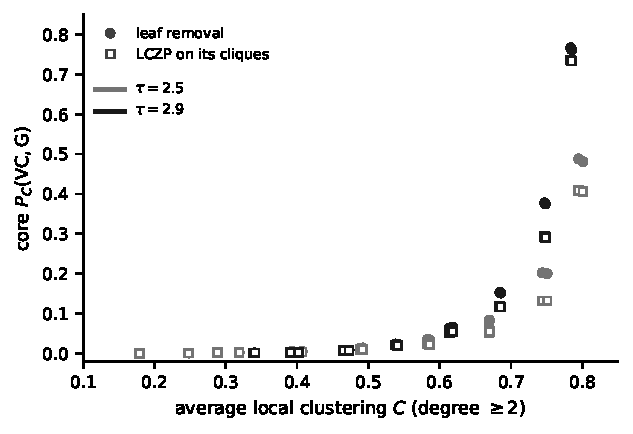
\includegraphics[width=\linewidth]{figs/fig-hrg-c.pdf}
\caption{\textbf{Vertex cover core size of hyperbolic random graphs.} The
leaf-removal core of hyperbolic random graphs against their own clustering,
both tails in one panel and both axes linear, $n=2\times10^{5}$ and two seeds
per point. Filled circles are leaf removal run on the graph; open squares are
the LCZP map evaluated on the maximal-clique ensemble measured from that same
graph, so nothing is fitted. The abscissa is the average local clustering over
vertices of degree at least two, which is where a triangle is possible at all:
these graphs are almost all isolated vertices at the sparse end --- under half
a per cent have two neighbours at $\ave{k}=0.05$ --- so the unrestricted mean
would report the density and call it clustering. The degree-matched
configuration model is not plotted: it sits at $C\le0.017$, off the left of the
axis, and has no core anywhere except at $\ave{k}=6$, $\tau=2.9$; the text
gives its numbers. Transitivity was tried
first and is not usable here: on a $\tau=2.5$ tail a few hubs of degree
$10^{3}$ set its denominator, and it comes out flat in $\ave{k}$ and split by
seed. Data from
\code{statmech/\allowbreak probe/\allowbreak hrg\_\allowbreak transitivity.\allowbreak py}
joined to
\code{statmech/\allowbreak probe/\allowbreak prediction4.\allowbreak py};
generated by
\code{figs/\allowbreak cover.\allowbreak py:figure\_\allowbreak hrg\_\allowbreak c}.}
\label{fig:hrgc}
\end{figure}

\paragraph{What the figure is drawn against.} Mean degree is the knob, and
Fig.~\ref{fig:hrgc} is drawn against what the knob produces instead, because
the separation this section is about is a separation in \emph{structure}. Every
hyperbolic graph in it sits between $C=0.18$ and $0.80$; every degree-matched
control sits at $C\le0.017$, which is why the control is not plotted --- on a
linear axis it would be a column of points on the ordinate.
What is plotted is the comparison that could have failed: the LCZP prediction
against the measurement, over the whole range, and the open squares follow the
filled circles at every clustering, recovering $64$ to $85$ per cent of the
measured core at $\tau=2.5$ and $77$ to $100$ at $\tau=2.9$. The gap is the
overlap deficit and it does not grow with $C$.

Two cautions come with it. Clustering is not a control here: it is produced by
$\ave{k}$, rising monotonically with it because a denser hyperbolic graph has
more vertices with two neighbours to be clustered, so this is a
reparametrisation of the density sweep and not an independent one. And at
$\ave{k}=6$ the control has a core of its own, $0.62$ at $C\approx0$ --- density
alone makes one, the point Sec.~\ref{sec:realcore} makes again on real
networks, and a reminder that the abscissa does not order the physics by
itself.

\paragraph{How much this establishes.} Less than it looks.
Section~\ref{sec:corefree} shows that \emph{any} layer of
cardinality three or more removes the core-free branch, so a positive prediction
follows from the algebra the moment one triangle enters the ensemble, whatever
else the graph is doing. The existence of the core was never in doubt once the
mapping was chosen.

The exponent is the part that could have failed. And there the evidence is
weaker than the central values suggest. Bootstrapped over seeds, the predicted
exponent does not move with $\tau$ at all --- $1.57$, $1.55$, $1.57$ at
$\tau=2.1$, $2.5$, $2.9$ --- while the measured one spreads by seven times as
much and rises monotonically with the tail, $1.49$, $1.59$, $1.64$. The two
agree within errors at $\tau=2.5$ and differ at $\tau=2.9$ by roughly four standard
deviations. What the comparison establishes is that the chygraph produces a
power law of about the right exponent; not that it tracks the exponent's
dependence on the tail. A sharper test would need an ensemble in which the
predicted exponent is made to move, and an analytic account of what fixes it
near $1.57$ in the LCZP map. Neither is attempted here, and both are on
Chapter~\ref{ch:outlook}'s list.

\section{Graphs with degree correlations}
\label{sec:vw}
\index{degree correlations}

Section~\ref{sec:hrg} ended on the claim that whatever separates the hyperbolic
graph from its degree-matched control is not in $\{p_{d},e_{dd'}\}$. That is a
statement about a description, and it is worth knowing what that description
\emph{can} do before concluding it cannot do this. It can do a great deal. Run
vertex cover over the full node-and-link ensemble --- arbitrary degree
distribution, arbitrary correlation between the degrees at the two ends of a
link --- and there is a phase transition along the correlation axis alone, with
the degree distribution held exactly fixed. It is due to \citet{vazquez2003vw},
and it is recapitulated here for two reasons. It fixes what the node-and-link
description is capable of, which Sec.~\ref{sec:hrg} needs in order to say that
the hyperbolic graph and its control are not separated by it. And it is this
chapter's own map, refined on a different index.

\paragraph{The ensemble.} Fix $p_{d}$, and with it the excess-degree
distribution $q_{d}=(d+1)p_{d+1}/\ave{k}$. Then fix, independently, the
symmetric joint distribution $e_{dd'}$ of the excess degrees at the two ends of
a link, subject only to $\sum_{d'}e_{dd'}=q_{d}$, so that the conditional
$p(d'|d)=e_{dd'}/q_{d}$ is what a walker arriving at a vertex of excess degree
$d$ sees on the other side. Uncorrelated graphs are the single point
$e_{dd'}=q_{d}q_{d'}$; everything else on that simplex is a correlated graph
with the \emph{same} degree distribution. This is the largest ensemble whose
atoms are nodes and links, and no further refinement of that vocabulary reaches
past it.

\paragraph{What it costs.} A Bethe--Peierls treatment on such a graph no longer
closes on one cavity-field distribution. It closes on one \emph{per excess
degree}, $P_{d}(h)$, coupled through $p(d'|d)$, because two vertices of the same
degree stop being statistically alike once the degrees of their neighbours
differ. In the $\mu\to\infty$ limit --- the hard-field limit of
Sec.~\ref{sec:hard}, and the same discard Sec.~\ref{sec:hardfail} shows is
harmless on a graph and fatal above cardinality two --- those distributions
collapse onto integers, and one scalar per degree class survives:
\begin{equation}
  \pi_{d}=\sum_{d'}\frac{e_{dd'}}{q_{d}}\,(1-\pi_{d'})^{\,d'},
  \label{eq:vwpi}
\end{equation}
with $\pi_{d}$ the probability that a link entering a vertex of degree $d+1$ is
not already covered from the other end. The cover size follows,
\begin{equation}
  x_{c}=1-p_{0}-\sum_{d\ge1}p_{d}\,(1-\pi_{d-1})^{\,d-1}
        \Bigl(1+\frac{d-2}{2}\,\pi_{d-1}\Bigr).
  \label{eq:vwxc}
\end{equation}

Equation~\eqref{eq:vwpi} is Eq.~\eqref{eq:vc} with the index moved. This
chapter resolves the one scalar $\sigma$ by \emph{layer}, because a node reached
along a layer-$m$ inclusion is size-biased in layer $m$ alone;
Eq.~\eqref{eq:vwpi} resolves it by \emph{degree class}, because a link entering
a vertex of excess degree $d$ lands on a neighbourhood biased by $p(d'|d)$. Two
refinements of one map, on two indices, and they are orthogonal: neither
reaches the other. Both are order-reversing, so both need Sec.~\ref{sec:hard}'s
bracket rather than plain iteration, and it was on this map that the
oscillation was first noticed and read as the physical signal it is.

At $e_{dd'}=q_{d}q_{d'}$ the sum in Eq.~\eqref{eq:vwpi} loses its $d$
dependence and the whole thing is one scalar again. For Poisson $p_{d}$ that
scalar is Sec.~\ref{sec:twoconstraints}'s: Eq.~\eqref{eq:vwxc} returns the
Weigt--Hartmann size to machine precision at $\ave{k}=1,2,3,5,10$, and its
instability sits at $\ave{k}=e$ to fifteen digits. Section~\ref{sec:onepoint}'s
one point with three names is the uncorrelated Poisson corner of this ensemble.

\begin{figure}[tbp]
\centering
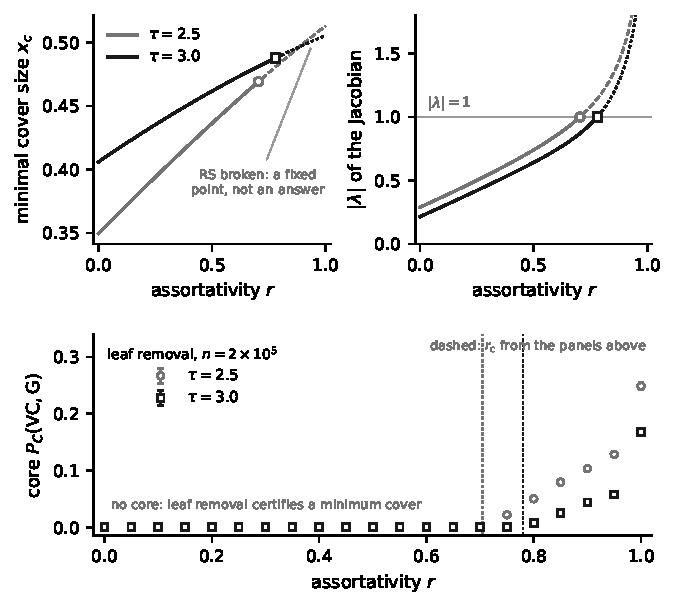
\includegraphics[width=\linewidth]{figs/fig-vw.pdf}
\caption{\textbf{Phase transition in degree correlated graphs.} Along the
assortativity axis of Eq.~\eqref{eq:vwr}, at $p_{d}\sim d^{-\tau}$ held
\emph{exactly} fixed: only $e_{dd'}$ moves. \emph{Top left}, the cover size,
solid where the fixed point of Eq.~\eqref{eq:vwpi} is stable and dashed past
$r_{\mathrm{c}}$ where it is a fixed point and not an answer. \emph{Top right},
the diagnostic \citet{vazquez2003vw} had to read off a failure to converge ---
the leading eigenvalue of the Jacobian there, crossing $1$. \emph{Below}, the
independent check: $P_{C}(\mathrm{VC},\mathrm{G})$ from leaf removal on graphs
drawn from the same ensemble by that paper's own generator, $n=2\times10^{5}$,
three seeds. Nothing is fitted and no chygraph is involved --- the dashed
verticals are $r_{\mathrm{c}}$ carried over from above. Data from
\code{statmech/\allowbreak probe/\allowbreak vw\_\allowbreak core.\allowbreak py};
generated by
\code{figs/\allowbreak cover.\allowbreak py:figure\_\allowbreak vw}.}
\label{fig:vw}
\end{figure}

\paragraph{The transition.} Move off that corner along
\begin{equation}
  e_{dd'}=q_{d}\bigl[\,r\,\delta_{dd'}+(1-r)\,q_{d'}\,\bigr],
  \label{eq:vwr}
\end{equation}
which runs from uncorrelated at $r=0$ to fully assortative at $r=1$ --- every
link joining equal degrees --- and preserves $q_{d}$, hence $p_{d}$, exactly at
every $r$. On scale-free degrees $p_{d}\sim d^{-\tau}$, $d\ge1$, the cover size
rises monotonically with $r$ and the fixed point of Eq.~\eqref{eq:vwpi} loses
stability, as in Fig.~\ref{fig:vw}, at
\begin{equation}
  r_{\mathrm{c}}=0.70\quad(\tau=2.5),
  \qquad
  r_{\mathrm{c}}=0.7802\quad(\tau=3.0),
  \label{eq:rc}
\end{equation}
the heavier tail breaking first. Below $r_{\mathrm{c}}$ the replica-symmetric
$x_{c}$ is the minimum cover size; above it, it is a fixed point and not an
answer. Over $0\le r\le0.7$ the size runs from $0.4059$ to $0.4810$ at
$\tau=3.0$ and from $0.35$ to $0.47$ at $\tau=2.5$ --- a fifth and a third ---
and nothing but the correlations has moved.

The transition is this chapter's, not a new one.
\citet{vazquez2003vw} ran generalised leaf removal on graphs drawn from
Eq.~\eqref{eq:vwr} at $n=10^{6}$ and tracked its certified error: it vanishes
with $n$ below $r_{\mathrm{c}}$, stays finite above it at any size, and the
onset coincides with the loss of stability. The lower panel of
Fig.~\ref{fig:vw} asks the same question of the object this chapter actually
computes, the core: leaf removal on graphs drawn from Eq.~\eqref{eq:vwr}
returns $P_{C}(\mathrm{VC},\mathrm{G})=0$ at every $r$ below $r_{\mathrm{c}}$
and a positive core above it, with the onset bracketed between the grid points
either side of $r_{\mathrm{c}}$ --- $0.70$ and $0.75$ at $\tau=2.5$, $0.75$
and $0.80$ at $\tau=3.0$, against $0.7042$ and $0.7802$ from
Eq.~\eqref{eq:rc}. \emph{Leaf removal certifies exactly where the hard-field
map is stable} --- Sec.~\ref{sec:onepoint}'s sentence, on an axis that section
never moves along, reached from a measurement rather than from algebra, and an
independent instance of the identification the chapter is built on.

\paragraph{Why Sec.~\ref{sec:hrg}'s control is still a control.} The reading
to block is that degree correlations are a small effect and clustering a large
one. They are not small: Eq.~\eqref{eq:vwr} moves the cover size by a third and
changes the phase, at frozen $p_{d}$. The point is a different one. The
hyperbolic graph and its degree-matched configuration model agree on $p_{d}$
\emph{and} on assortativity to within a few per cent, so they do not merely
share a degree distribution --- they sit at the same place on the surface
Eq.~\eqref{eq:vwpi} is solved over, and far inside its replica-symmetric region
on both counts. One of them has an extensive core at every density down to
$\ave{k}=0.05$; the other has none until $\ave{k}$ reaches $4.5$ to $10$. The
axis this section exercises carries a transition, and the two graphs are not
separated along it. Chapter~\ref{ch:introduction}'s claim is therefore not that
degree correlations do nothing, but that this pair of graphs differs in
something the pair $\{p_{d},e_{dd'}\}$ does not record.

\begin{figure}[tbp]
\centering
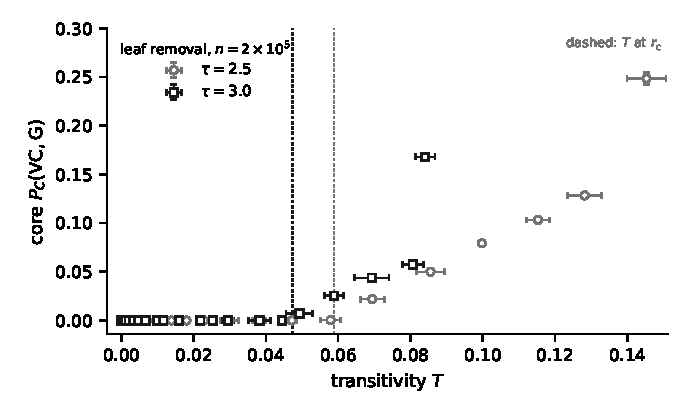
\includegraphics[width=\linewidth]{figs/fig-vw-t.pdf}
\caption{\textbf{Order parameter vs transitivity.}
Figure~\ref{fig:vw}'s measured core replotted with transitivity on the
abscissa, $T$ measured on the same graphs, and the verticals $T$ at
$r_{\mathrm{c}}$ carried across by the monotone $T(r)$. Turning $r$ makes
triangles, and the core arrives with them. It does not arrive at the same
number of them in the two tails --- $T=0.0589$ against $0.0474$, a wider spread
than the $r_{\mathrm{c}}$ it came from --- so transitivity is not the
coordinate the transition is simple in. $T$ is an outcome of $r$ and not a
control: nothing here holds it fixed. Generated by
\code{figs/\allowbreak cover.\allowbreak py:figure\_\allowbreak vw\_\allowbreak t}.}
\label{fig:vwt}
\end{figure}

\paragraph{Turning $r$ also makes triangles.} The axis is therefore not a
pure correlation axis. At $\tau=2.5$ and $n=2\times10^{5}$ the transitivity of
the drawn graphs runs from $1.6\times10^{-4}$ at $r=0$ to $0.145$ at $r=1$, and
the mechanism is starvation: a high-degree node may attach only within its own
degree class, the tail has few members to offer, and the classes saturate into
small dense blocks --- the fraction of stub pairings discarded as a repeat or a
self-loop climbs from $0$ to $0.075$ in step. So Eq.~\eqref{eq:vwr} does not
move along $e_{dd'}$ with everything else held fixed, and
Fig.~\ref{fig:vwt} is Fig.~\ref{fig:vw}'s core asked again against $T$. The
core arrives with the triangles, which is Sec.~\ref{sec:corefree}'s statement
turning up in an ensemble that was not built to make any; but it does not
arrive at the same $T$ in the two tails, $0.0589$ against $0.0474$ where
$r_{\mathrm{c}}$ was $0.7042$ against $0.7802$, a wider spread and not a
narrower one. Transitivity therefore orders the approach to the transition but
does not locate it.

This does not rescue $\{p_{d},e_{dd'}\}$, and Sec.~\ref{sec:hrg}'s reading
survives it for two reasons. The clustering arrives only at extreme
assortativity, and the hyperbolic graph and its control both sit near $r=0$,
where this ensemble's $T$ is $10^{-4}$ against the $10^{-1}$ the geometry
supplies. And it arrives on the \emph{hubs}: average local clustering, which is
Chapter~\ref{ch:data}'s $C$, rises with $r$ but vanishes as $n^{-0.4}$ at every
$r$, so almost no vertex is in a triangle even where triples are. What the
paragraph does establish is that the correlation axis carries clustering with
it, which has to be known before it is used as a null.

\paragraph{What is added here is a diagnosis, not a result.} The instability
was originally located by watching the iteration fail to converge, which is a
real signal --- the map is order-reversing, so an unstable fixed point gives a
period-two orbit and not a drift --- but it is one instrument doing two jobs,
and it cannot report a fixed point it has failed to reach. Under
Eq.~\eqref{eq:vwr} the map closes on the single scalar
$\sum_{d}q_{d}(1-\pi_{d})^{\,d}$, so nested bisection reaches the fixed point on
either side of $r_{\mathrm{c}}$ and stability is then asked of the Jacobian
there; that Jacobian is diagonal plus rank one, so its spectrum comes from a
secular equation rather than an eigensolve, and is cross-checked against one.
The algebra is in \code{vertexcover.\allowbreak py} and
Eq.~\eqref{eq:rc} is produced by
\code{statmech/\allowbreak examples/\allowbreak vw03\_\allowbreak figure1.\allowbreak py}.
The digits carry a caveat. At $\tau=3.0$ they are converged in the degree
cutoff and at $\tau=2.5$ they are not, since $\ave{k}$ itself converges slowly
against a $2.5$ tail: two decimals are real there and four at $\tau=3.0$, which
is why Eq.~\eqref{eq:rc} quotes them to different precision.

\section{Real networks}
\label{sec:realcore}
\index{leaf removal}
\index{core}

Section~\ref{sec:hrg} tested the LCZP map on an ensemble built to be
clustered. This section runs the same comparison on sixteen real
networks: the ten of Chapter~\ref{ch:data}'s
Table~\ref{tab:real} and the six Chapter~\ref{ch:overlap} works with, read from
the same cache. That chapter keeps to induced neighbourhoods of at most twenty
vertices because it enumerates $\ln Z$; leaf removal is linear, so whole
networks are used here.

The two columns are the same quantity by two routes. \emph{Leaf removal on
the graph} is the measurement, $P_{C}(\mathrm{VC},\mathrm{G})$. \emph{LCZP on
its cliques} is the prediction, $P_{C}(\mathrm{VC},\chi)$, evaluated on the
maximal-clique ensemble measured from that same graph, with nothing fitted.
What is being asked is whether the second reproduces the first --- whether
knowing a real network's degree distribution and its cliques is enough to say
how much of it leaf removal will fail on. Why the cliques should matter at all
is settled before this section and not in it: Sec.~\ref{sec:corefree} shows
algebraically that a complex of three or more members destroys the core-free
branch, and Sec.~\ref{sec:hrg} shows it on an ensemble where the clustering can
be turned against a degree-matched control. Triangles make covering hard; the
question here is how well the map counts them.

\begin{table}[t]
\centering\small
\begin{adjustbox}{max width=\linewidth}
\begin{tabular}{lrrrrr}
\hline\hline
 & & & \multicolumn{3}{c}{core fraction}\\
network & $\ave{k}$ & $C$ & leaf removal & Eq.~\eqref{eq:core} & leaf removal\\
 & & & on the graph & on its cliques & rewired\\
\hline
Euroroad & 2.51 & 0.019 & 0.1559 & 0.0162 & 0.0111\\
PDZ domains & 2.60 & 0.007 & 0.0248 & 0.0014 & 0.0000\\
Power grid & 2.67 & 0.080 & 0.0927 & 0.0337 & 0.0005\\
Yeast (Y2H) & 2.67 & 0.071 & 0.0405 & 0.0157 & 0.0000\\
C. elegans 2007 & 2.71 & 0.017 & 0.0000 & 0.0007 & 0.0000\\
C. elegans WI8 & 3.20 & 0.022 & 0.0000 & 0.0008 & 0.0000\\
Human (Stelzl) & 3.85 & 0.006 & 0.0000 & 0.0002 & 0.0002\\
Human (Vidal) & 4.32 & 0.072 & 0.0313 & 0.0056 & 0.0000\\
Co-authorship & 4.82 & 0.741 & 0.6385 & 0.7101 & 0.5983\\
Human (Figeys) & 5.79 & 0.040 & 0.0000 & 0.0010 & 0.0000\\
Les Mis. scenes & 6.60 & 0.573 & 0.5065 & 0.4731 & 0.2909\\
Football & 10.66 & 0.403 & 1.0000 & 1.0000 & 1.0000\\
Facebook & 11.88 & 0.605 & 0.8085 & 0.8444 & 0.8020\\
Collins yeast & 16.57 & 0.648 & 0.7490 & 0.7798 & 0.7129\\
Jazz bands & 27.70 & 0.617 & 0.9495 & 0.9561 & 0.9487\\
Hospital contacts & 30.37 & 0.640 & 1.0000 & 1.0000 & 1.0000\\
\hline\hline
\end{tabular}

\end{adjustbox}
\caption{\textbf{Leaf removal on sixteen real networks.} The core fraction by
two routes: $P_{C}(\mathrm{VC},\mathrm{G})$ from leaf removal run on the
graph, and $P_{C}(\mathrm{VC},\chi)$ from the LCZP map, Eq.~\eqref{eq:core}, on
that graph's own maximal-clique ensemble. $C$ is the clustering coefficient.
Ordered by mean degree, which is what sorts the rows into the three groups the
text takes them in. Generated by
\code{figs/\allowbreak cover.\allowbreak py:table\_\allowbreak real\_\allowbreak core} from
\code{statmech/\allowbreak probe/\allowbreak real\_\allowbreak core.\allowbreak py}.}
\label{tab:realcore}
\end{table}

\begin{figure}[tbp]
\centering
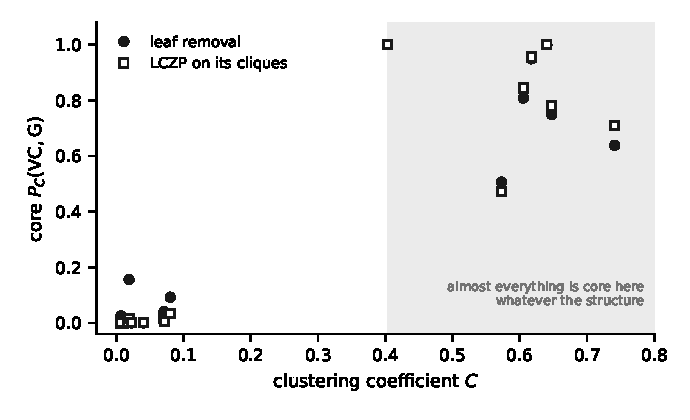
\includegraphics[width=\linewidth]{figs/fig-real-core.pdf}
\caption{\textbf{Core size against clustering for sixteen real networks.}
Table~\ref{tab:realcore}'s two core columns
against its clustering column: leaf removal on the graph, and the LCZP map on
that graph's own maximal cliques. The shading is not a third measurement. It
marks the seven networks that are already more than half core --- $0.51$ to
$1.00$, at $\ave{k}$ from $4.8$ to $30.4$ --- where returning \emph{nearly all
of it} is agreement won for free, and where the two symbols therefore sit on
top of each other. Everything the section rests on is to the left of it, and it
is compressed into the first eighth of the axis, which is the other thing the
figure is showing. Generated by
\code{figs/\allowbreak cover.\allowbreak py:figure\_\allowbreak real\_\allowbreak core}
from
\code{statmech/\allowbreak probe/\allowbreak real\_\allowbreak core.\allowbreak py}.}
\label{fig:realcore}
\end{figure}

Figure~\ref{fig:realcore} draws the table, and its shape is the warning this
section has to give before any of its numbers are read. Core rises with
clustering across the sixteen, which is the result one would like to have; but
the networks with high $C$ are also the dense ones, and a curve drawn through
the figure as a whole would be measuring $\ave{k}$. The evidence is the nine
points crowded against the ordinate, at $C\le0.08$, where the graph is sparse
enough that having a core is not automatic. The paragraphs below take the
sixteen in three groups for that reason.

\paragraph{Seven networks are already more than half core.} They run from
$0.51$ to $1.00$, at $\ave{k}$ from $4.8$ to $30.4$, and at those densities
almost every vertex is in the $2$-core before any question of clustering
arises. The chygraph tracks the measurement there --- $93$ to $111$ per cent of it
--- and that agreement establishes nothing, because a constant would have done
as well. Density is not sorted by $\ave{k}$ alone, which is why the group
is defined by the core and not by the degree: the Figeys interactome sits at
$\ave{k}=5.8$ with no core at all.

\paragraph{Five carry the comparison.} Euroroad, the PDZ and Yeast two-hybrid
interactomes, the power grid and the Vidal screen are sparse --- $\ave{k}$ from
$2.5$ to $4.3$, four of them below the Poisson threshold $\ave{k}=e$ of
Sec.~\ref{sec:onepoint} --- and all five have a core, from $0.025$ on PDZ to
$0.156$ on Euroroad. The chygraph built from their cliques predicts one on
every one of them. That threshold is a Poisson number and these degree
distributions are not Poisson, so it does not by itself say the degree
distribution could not have produced these cores; what settles that is
Sec.~\ref{sec:corefree} algebraically and Sec.~\ref{sec:hrg} on an ensemble
where the clustering can be varied at fixed degree distribution. What the five
add is that the prediction is evaluated on measured clique ensembles, with
nothing fitted, and returns a core where there is one.

\paragraph{Quantitatively it is much worse than on hyperbolic graphs.} Those
five recover $5.8$ to $38.8$ per cent of the measured core, where
Sec.~\ref{sec:hrg} recovered $77$ to $100$. The direction of the error is the
same --- the chygraph understates --- and so, presumably, is the cause, since
these are the sparsest networks in the set and Chapter~\ref{ch:data} measured
their $\mathrm{shared}_{2+}$ at $0.000$ to $0.022$: the cliques of a real
network share vertices, the map assumes they do not, and the sharing is what it
throws away. On a real network that cannot be established the way
Sec.~\ref{sec:hrg} establishes it, since the clique ensemble cannot be
rearranged with everything else held fixed. The direction is what is reported.

\paragraph{Four networks have no core at all, which is what
Sec.~\ref{sec:corefree} predicts.} The two \emph{C. elegans} screens and the
Stelzl and Figeys interactomes return exactly zero, and the LCZP map
returns between $2\times10^{-4}$ and $1\times10^{-3}$ on them. Both are right.
Section~\ref{sec:corefree} proves the core cannot vanish identically once any
complex of three or more members is present, and the paragraph that blocks the
strong reading of it says precisely this case: non-zero as the algebra requires,
and too small to see. A prediction of $10^{-4}$ on a graph of two thousand
vertices is a prediction of no core, and no core is what leaf removal finds.

\paragraph{What this adds to Sec.~\ref{sec:hrg}.} Less than the sixteen rows
suggest, and in one respect more. Eleven of the sixteen are uninformative ---
seven because almost everything is core, four because nothing is. The five that
carry the comparison agree with the hyperbolic result in direction and are
three to ten times worse in magnitude. What is new is the paragraph before
this one: the weak form of Sec.~\ref{sec:corefree}, that the core is non-zero
but can be negligible, was argued there from a constructed example with a
triangle layer of chy-degree $10^{-3}$, and here it is four real networks.

\paragraph{Three ensembles, one conclusion.} The chapter has now put the same
question to three families of graph that share no construction. Hyperbolic
graphs are clustered by the geometry they are built in, and carry a core at
every density down to $\ave{k}=0.05$ (Sec.~\ref{sec:hrg}). The correlated
graphs of Sec.~\ref{sec:vw} acquire triangles as a side effect of
assortativity, and their core appears where those triangles do. These sixteen
are clustered by whatever the data recorded, and the five sparse enough for the
question to be open have a core as well. The mechanism is the same in the three
cases and is stated in Sec.~\ref{sec:corefree}: above cardinality two the
core-free branch does not exist, so one layer of triangles is enough to remove
it. The three ensembles do not prove that --- the algebra does --- but they are
the three cases in which the prediction was made against structure the model
did not choose.

\section{Checks}
\label{sec:cover-checks}

\checkhead{Known results}
The $c=2$ threshold returns $e$ to ten digits, which is Bauer--Golinelli.
Equation~\eqref{eq:vc} at $c=2$ returns the Weigt--Hartmann cover size, agreeing
with Eq.~\eqref{eq:hs} to nine digits along a different code path.
Section~\ref{sec:vw} is a recapitulation of \citet{vazquez2003vw} and adds no
result: Eq.~\eqref{eq:vwxc} at $e_{dd'}=q_{d}q_{d'}$ and Poisson $p_{d}$
returns the Weigt--Hartmann size to machine precision at $\ave{k}=1,2,3,5,10$,
and the instability of Eq.~\eqref{eq:vwpi} at the same point returns $e$ to
fifteen digits --- a third independent route to Sec.~\ref{sec:onepoint}'s
number. The secular criterion behind Eq.~\eqref{eq:rc} and
Fig.~\ref{fig:vw} is cross-checked against a dense eigensolve of the same
Jacobian, and agrees to $8\times10^{-15}$. Figure~\ref{fig:vw}'s lower panel is
a measurement and not a recapitulation: leaf removal on graphs drawn from
Eq.~\eqref{eq:vwr} at $n=2\times10^{5}$, three seeds, brackets the onset of the
core between the grid points either side of Eq.~\eqref{eq:rc}'s
$r_{\mathrm{c}}$ at both tails, with the core zero to $4\times10^{-4}$ below
and rising steeply above. That the core and the loss of stability coincide on
the \emph{correlation} axis does not follow from Sec.~\ref{sec:onepoint}, which
establishes it on the chy-degree axis, and it is checked here rather than
assumed. The grid is $\Delta r=0.05$, so the bracket is all the resolution
claimed; no finite-size scaling of the onset was done. Figure~\ref{fig:vwt}
reparametrises that measurement and adds no data. Its abscissa is an outcome
and not a control, and it is not clean in $n$: transitivity is flat in system
size at $\tau=2.5$, drifting as $n^{-0.02}$ to $n^{-0.05}$ over a decade, but
falls as $n^{-0.15}$ at $\tau=3.0$, so at larger $n$ that curve would slide
left and the threshold spread would widen rather than close. The clustering
figures quoted with it --- $T$ against $r$, average local clustering vanishing
as $n^{-0.4}$, and the discarded-pairing fraction --- are from
\code{statmech/\allowbreak probe/\allowbreak vw\_\allowbreak clustering.\allowbreak py}
at three sizes and two seeds, which is enough for the exponents to two figures
and no more.

\checkhead{New results}
The identification of the three points, everything above cardinality two, and
the hyperbolic-graph and real-network tests are new here. On the four real
networks with no measured core, the LCZP map returns between
$2\times10^{-4}$ and $1\times10^{-3}$, which is Sec.~\ref{sec:corefree}'s weak
form --- non-zero and negligible --- met in data rather than in the constructed
example that paragraph uses. Equation~\eqref{eq:factored} is an
identity, checked symbolically; the numerical map agrees, reporting a core-free
branch at $c=2$ and none at $c=3,4,5,8$, and that the core is exactly
$1-e^{-\ave{k}}$ above cardinality two is checked against the closed form at
three cardinalities and three densities. The core-percolation threshold and the
hard-field instability of Chapter~\ref{ch:hittingset}, computed independently,
agree to $2.5\times10^{-10}$. The LCZP map is compared with pure
leaf removal on graphs built to match it, at $n=4\times10^{5}$, over eleven
ensembles at cardinalities two, three and four, with an error running from
$8.7\times10^{-5}$ to $3.1\times10^{-3}$. The multi-layer threshold
Eq.~\eqref{eq:corethresh} returns Eq.~\eqref{eq:sumkappae}'s total chy-degree
$e$ to $2\times10^{-10}$ at one, two, three and five Poisson layers, evenly and
unevenly split. Equation~\eqref{eq:vcinstab} is checked by evaluating the
instability of Eq.~\eqref{eq:vc} at its own root, which returns $1$ to ten
digits at $c=2,\dots,10$. Equation~\eqref{eq:smallcore} agrees with the
numerical map to $10^{-4}$ relative or better at $c=3,4,5,8$ and three link
densities, and reproduces the $1.8\times10^{-4}$ of
Sec.~\ref{sec:corefree}'s constructed example. Table~\ref{tab:five} recomputes
nothing: each row is Eq.~\eqref{eq:vc} and Eq.~\eqref{eq:core} on one list of
cardinalities, and its three cardinality-two rows agree with each other, and its
hypergraph rows with the closed form $1-\Phi(0)$, to every digit printed.

\checkhead{Partial results}
Section~\ref{sec:realcore} establishes less than sixteen rows suggest, and the
text says which rows carry it. Seven of the networks are already more than half
core, so a prediction of nearly all of it agrees for free; four have no core at
all. Five carry it, and on those the chygraph recovers $5.8$ to $38.8$ per cent
of the measured core against Sec.~\ref{sec:hrg}'s $77$ to $100$ --- the same
direction, three to ten times worse. The overlap that
Sec.~\ref{sec:hrg} identifies as the cause by rearranging its ensemble cannot
be isolated that way on a real network, so the direction is reported and the
attribution is carried over rather than remeasured.
Section~\ref{sec:vw}'s digits are not all converged: at $\tau=2.5$ the
degree cutoff still moves $r_{\mathrm{c}}$ and $x_{c}$ in the third decimal,
because $\ave{k}$ itself converges slowly against that tail, so two decimals
are quoted there against four at $\tau=3.0$. None of the structural claims ---
the ordering of the two curves, monotonicity in $r$, replica symmetry at $r=0$
--- depends on that, and the published figure has not been digitised, so the
agreement with it is structural and not numerical.
Figure~\ref{fig:hrgc} recomputes no core: it is
\code{prediction4}'s columns joined to the clustering of the same graphs,
measured on regenerated copies at the same seeds and calibration, and its
abscissa is produced by $\ave{k}$ rather than varied against it. Transitivity
was measured first and rejected: on these tails it is flat in $\ave{k}$ and
separated by seed --- $0.009$ to $0.011$ against $0.016$ to $0.021$ at
$\tau=2.5$ --- because a few hubs of degree $10^{3}$ own its denominator, and
the rejection is recorded here because the same coordinate does work in
Sec.~\ref{sec:vw}, where the degrees are bounded by the cutoff and the
triangles are on the hubs by construction.
Section~\ref{sec:hrg} establishes less than its numbers suggest, and both
qualifications are carried in the text. The
\emph{existence} of the core follows from the algebra the moment a single
triangle enters the ensemble, so it was never at risk. Only the exponent could
have failed, and there the predicted value does not move with the tail while the
measured one does: they agree within errors at $\tau=2.5$ and differ at
$\tau=2.9$ by roughly four standard deviations. What lies past $\ave{k}=e$ --- the
complexity, and the one-step answer for this family --- is not computed here.
